\subsection{A New Parallel Blockchain Construction}
\label{subsec:new-parallel-blockchain}

We describe how parallel blockchains can be run continuously for any (polynomially bounded) number of intervals, thus allowing Weak/Approximate Agreement protocols (and later clock synchronization and Byzantine agreement) to be sequentially invoked.

The PoW-based Approximate Agreement protocol presented in~\cref{subsec:apa-honst-majority} terminates in constant time, and the security of an invocation relies on a high-entropy CRS to invalidate all RO queries made by corrupted parties before the activation of honest parties (a.k.a. pre-mining attack).
%
Nonetheless, since CRS is available only at the beginning of the first invocation, sequentially running multiple invocations of \cref{protocol:approximate-consensus} does not provide any security guarantee for the second and later invocations.
%
More precisely, the na\"ive sequential composition of AA protocols, by keep extending $m$ separate chains and let online parties periodically update their internal state based on the blocks on the tip of the chains in their local view, incurs the following problem:
%
Since any interval might be ``reverted'' in the future as the adversary manages to create a longer fork and surpass the current one, parties that join after the beginning of an execution cannot synchronize with the online parties, as a large fraction of chains that online parties used to synchronize their clocks will get orphaned in the future.

To tackle this problem, we introduce a novel parallel blockchain construction, which we later show supports the following features:
%
(i) it enables interval-based state update, thus parties update their internal state at the end of each interval;
%
(ii) it has no dependency on a global clock and can self-synchronize all parties' local clocks as long as they proceed at some bounded rates;
%
and (iii) it allows difficulty adjustment thus supports dynamic participation while preserving the optimal corruption resiliency.

The main difference between our parallel blockchain construction and that employed by Chain-King Consensus in~\cite{EC:GarKiaShe24} is that, in~\cite{EC:GarKiaShe24} it requires a chain to be ``dense'' such that it possesses sufficiently many blocks in any time window of fixed length in an interval, and each chain should point to sufficiently many dense chains in the previous interval (i.e., cross chain reference).
%
Contrary, in our construction we completely eliminate the hardcoded density parameter and the cross chain references, hence switching from the ``fragmented'' chain structure to the ``continuous'' one.

\paragraph{Parallel blocktrees.}
%
We elaborate our construction now.
%
We extend the parallel chain structure to \emph{parallel blocktrees} consisting of $m$ independent blocktrees.
%
Recall that, on a single chain, all blocks on the same height competes with each other and only the one on the longest chain survives; thus blocks in the current view might get discarded from the longest chain in the future.
%
To help parties retrieve previously-longest yet now-orphaned forks, all blocks needs to be bookkeeped.
%
In this sense, a single chain is extended to a \emph{blocktree}.
%
The root of this tree is the genesis block and each path corresponds to one fork.
%
We note that this adaption is for future retrieval only, and parties still follow the heaviest (i.e., with most accumulated difficulty; longest in case of static participation) chain rule to select and process incoming chains.
%
In other words, parties adopt the heaviest fork in a blocktree and try to extend that fork using PoW, but they also bookkeep all forks.

A parallel blocktree is simply a parallel repetition of $m$ blocktrees whose mining procedure on the heaviest fork is bounded using \mforone PoW.
%
See \cref{fig:parallel-blocktree} for an illustration.
%
We also extend the blockchain notations to capture this modification.
%
Specifically, we write \blockTree denoting a blocktree.
%
I.e., a genesis block with no incoming edges and all other blocks are connected by an incoming edge from exactly one other block.
%
We write $\chain \in \blockTree$ if \chain matches one path in \blockTree.
%
Regarding parallel chains, let \parallelTrees denote $m$ parallel chains and we write $\parallelChains \in \parallelTrees$ if $\forall \chain \in \parallelChains$, it holds that $\chain \in \blockTree$ where \blockTree is the corresponding blocktree in \parallelTrees.

\begin{figure}[ht] \centering
    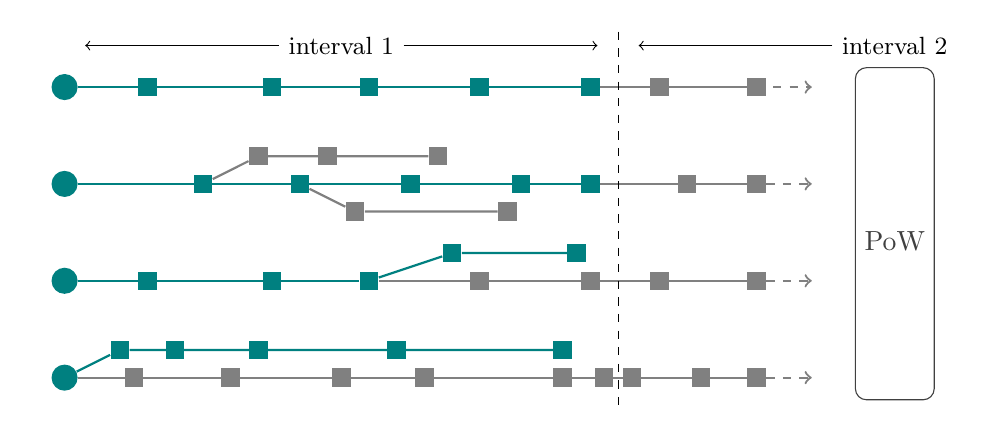
\begin{tikzpicture}
        \node (genesis) {};

        \node[fill = teal, circle] at ([xshift = 10pt, yshift = 50pt]genesis) (block11) {};
        \node[fill = teal] at ([xshift = 30pt]block11) (block12) {};
        \node[fill = teal] at ([xshift = 75pt]block11) (block13) {};
        \node[fill = teal] at ([xshift = 110pt]block11) (block14) {};
        \node[fill = teal] at ([xshift = 150pt]block11) (block15) {};
        \node[fill = teal] at ([xshift = 190pt]block11) (block16) {};
        \node[fill = gray] at ([xshift = 215pt]block11) (block17) {};
        \node[fill = gray] at ([xshift = 250pt]block11) (block1x) {};
        \draw[teal, thick] (block11) -- (block16);
        \draw[gray, thick] (block16) -- (block1x);

        \node[fill =  teal, circle] at ([xshift = 10pt, yshift = 15pt]genesis) (block21) {};
        \node[fill = teal] at ([xshift = 50pt]block21) (block22) {};
        \node[fill = teal] at ([xshift = 85pt]block21) (block23) {};
        \node[fill = teal] at ([xshift = 125pt]block21) (block24) {};
        \node[fill = teal] at ([xshift = 165pt]block21) (block25) {};
        \node[fill = teal] at ([xshift = 190pt]block21) (block26) {};
        \node[fill = gray] at ([xshift = 225pt]block21) (block27) {};
        \node[fill = gray] at ([xshift = 250pt]block21) (block2x) {};
        \draw[teal, thick] (block21) -- (block26);
        \draw[gray, thick] (block26) -- (block2x);
        \node[fill = gray] at ([xshift = 70pt, yshift = 10pt]block21) (block2f1) {};
        \node[fill = gray] at ([xshift = 95pt, yshift = 10pt]block21) (block2f2) {};
        \node[fill = gray] at ([xshift = 135pt, yshift = 10pt]block21) (block2f3) {};
        \draw[gray, thick] (block22) -- (block2f1) -- (block2f3);
        \node[fill = gray] at ([xshift = 105pt, yshift = -10pt]block21) (block2f4) {};
        \node[fill = gray] at ([xshift = 160pt, yshift = -10pt]block21) (block2f5) {};
        \draw[gray, thick] (block23) -- (block2f4) -- (block2f5);


        \node[fill =  teal, circle] at ([xshift = 10pt, yshift = -20pt]genesis) (block31) {};
        \node[fill = teal] at ([xshift = 30pt]block31) (block32) {};
        \node[fill = teal] at ([xshift = 75pt]block31) (block33) {};
        \node[fill = teal] at ([xshift = 110pt]block31) (block34) {};
        \node[fill = gray] at ([xshift = 150pt]block31) (block35) {};
        \node[fill = gray] at ([xshift = 190pt]block31) (block36) {};
        \node[fill = gray] at ([xshift = 215pt]block31) (block37) {};
        \node[fill = gray] at ([xshift = 250pt]block31) (block3x) {};
        \draw[teal, thick] (block31) -- (block34);
        \draw[gray, thick] (block34) -- (block3x);
        \node[fill = teal] at ([xshift = 140pt, yshift = 10pt]block31) (block3f1) {};
        \node[fill = teal] at ([xshift = 185pt, yshift = 10pt]block31) (block3f2) {};
        \draw[teal, thick] (block34) -- (block3f1) -- (block3f2);


        \node[fill =  teal, circle] at ([xshift = 10pt, yshift = -55pt]genesis) (block41) {};
        \node[fill = gray] at ([xshift = 250pt]block41) (block4x) {};
        \node[fill = gray] at ([xshift = 25pt]block41) (block42) {};
        \node[fill = gray] at ([xshift = 60pt]block41) (block43) {};
        \node[fill = gray] at ([xshift = 100pt]block41) (block44) {};
        \node[fill = gray] at ([xshift = 130pt]block41) (block45) {};
        \node[fill = gray] at ([xshift = 180pt]block41) (block46) {};
        \node[fill = gray] at ([xshift = 195pt]block41) (block47) {};
        \node[fill = gray] at ([xshift = 205pt]block41) (block48) {};
        \node[fill = gray] at ([xshift = 230pt]block41) (block49) {};
        \draw[gray, thick] (block41) -- (block4x);
        \node[fill = teal] at ([xshift = 20pt, yshift = 10pt]block41) (block4f1) {};
        \node[fill = teal] at ([xshift = 40pt, yshift = 10pt]block41) (block4f2) {};
        \node[fill = teal] at ([xshift = 70pt, yshift = 10pt]block41) (block4f3) {};
        \node[fill = teal] at ([xshift = 120pt, yshift = 10pt]block41) (block4f4) {};
        \node[fill = teal] at ([xshift = 180pt, yshift = 10pt]block41) (block4f5) {};
        \draw[teal, thick] (block41) -- (block4f1) -- (block4f5);

        \draw[black, dashed] ([xshift = 200pt, yshift = 20pt]block11.center) -- ([xshift = 200pt, yshift = -10pt]block41.center);
        \node at ([xshift = 100pt, yshift = 15pt]block11.center) (interval1) {\small interval 1};
        \draw[black, ->] (interval1.west) -- ([xshift = -70pt]interval1.west);
        \draw[black, ->] (interval1.east) -- ([xshift = 70pt]interval1.east);
        \node at ([xshift = 300pt, yshift = 15pt]block11.center) (interval2) {\small interval 2};
        \draw[black, ->] (interval2.west) -- ([xshift = -70pt]interval2.west);

        \node[darkgray, fill = white, draw = darkgray, rounded corners, minimum height = 120pt, align=center] at ([xshift = 50pt, yshift = -18pt]block2x) (pow) {\funcRO\\\mforone PoW};

        \draw[gray, thick, dashed, ->] (block1x.center) -- ([xshift = 20pt]block1x.center);
        \draw[gray, thick, dashed, ->] (block2x) -- ([xshift = 20pt]block2x.center);
        \draw[gray, thick, dashed, ->] (block3x) -- ([xshift = 20pt]block3x.center);
        \draw[gray, thick, dashed, ->] (block4x) -- ([xshift = 20pt]block4x.center);
    \end{tikzpicture}

    \caption{
        An illustration of the parallel blocktrees and the mining procedure.
        %
        Genesis blocks on each chain are represented as circles.
        %
        Teal blocks and forks depicts the view of a party at the end of the first interval.
        %
        There is no fork on the first chain; and on the second chain, forks are bookkeeped yet fail to revert the longest one.
        %
        The last two blocks in the view of a party on the third chain are discarded from the longest chain by another longer fork.
        %
        On the forth chain, all blocks in the first interval are reverted.
    }
    \label{fig:parallel-blocktree}
\end{figure}


\paragraph{Intervals and stages.}
%
We divide protocol time into consecutive, non-overlapping ``intervals'' in order to periodically let protocol participants adjust their local clocks and update internal states.
%
An interval consists of \syncLen rounds.
%
Parties decide which interval they are in based on their local time (thus different parties may stay in different intervals).
%
An interval is further divided into three consecutive, non-overlapping stages --- view convergence (\textsf{VC}), output generation (\textsf{OG}) and reference convergence (\textsf{RC}).
%
We denote their duration by $\syncLen_{\mathsf{VC}}$, $\syncLen_{\mathsf{OG}}$ and $\syncLen_{\mathsf{RC}}$ respectively.
%
In the view convergence (\textsf{VC}) stage, parties extend their local parallel chains and wait for the second stage.
%
Then, in the output generation (\textsf{OG}) stage, parties generate input-blocks which contain their suggested output value (cf.~\cref{subsec:new-smr-protocol}), local time (see~\cref{subsec:clock-sync-procedure}) and also interval retrieval information (see this section below).
%
They emit these input-blocks and record them on the blockchain.
%
Regarding the last stage \textsf{RC}, parties wait for a (possibly) common view of the \textsf{OG} stage and they adjust their clocks and update their internal state at the end of this stage (which is also the end of an interval).

\paragraph{A new timestamping scheme.}
%
Next, we introduce our new timestamping scheme for protocols to work with drifting clocks.
%
We extend the block timestamp from the conventional single round index $r \in  \mathbb{N}^+$ to a pair of both interval index and round index, i.e., $\protocolTime{itvl}{r} \in \mathbb{N}^+ \times \mathbb{N}^+$.
%
We say a block \block on a chain \chain is in interval $itvl$, if it reports a timestamp \protocolTime{itvl}{\cdot}.
%
A block $\block$ owns a valid timestamp iff. it satisfies the predicate $\mathsf{validTS}(r, itvl) \triangleq r \le itvl \cdot \syncLen$.
%
Note that this allows for a chain in interval $itvl$ to start with blocks reporting timestamps smaller than $(itvl - 1)\cdot \syncLen$.
%
Such adaption is necessary, since the clock adjustment algorithm might set clocks backwards; however, in the PoW setting parties must try to produce blocks in the next interval hence they should be able to mine with ``retorted'' timestamps.

Regarding blocks on the same chain (same fork on the blocktree), our protocol employs a new validation rule which asks for the monotonicity in the magnitude of stages.
%
To be precise, let $\mathsf{stage}: \mathbb{N}^+ \times \mathbb{N}^+ \rightarrow \mathbb{N}^+ \times \{ \mathsf{VC}, \mathsf{OG}, \mathsf{RC} \}$ be a function that takes a (valid) timestamp as input and outputs its corresponding stage.
%
We define a canonical order on $(itvl, stage) \in \mathbb{N}^+ \times \{ \mathsf{VC}, \mathsf{OG}, \mathsf{RC} \}$ as $(1, \mathsf{VC}), (1, \mathsf{OG}), (1, \mathsf{RC}), (2, \mathsf{VC}), (2, \mathsf{OG}), (2, \mathsf{RC}), \ldots$ so that operations like ``$<, =, \le$'' are defined canonically.
%
A chain \chain owns valid timestamps iff. for any two blocks $\block, \block'$ on \chain with timestamps \protocolTime{itvl}{r}, \protocolTime{itvl'}{r'} respectively, \block is an ancestor of $\block'$ implies $\mathsf{stage}(itvl, r) \le \mathsf{stage}(itvl', r')$.

In summary, our timestamp validation predicate, taking two consecutive blocks as input, is defined as follows.\footnote{A similar timestamping scheme with dual indices is proposed in~\cite{TCC:GarKiaShe22}. Yet their scheme still requires monotonically increasing timestamps within an interval while ours removes this restriction.}
%
\begin{equation} \label{eq:valid-timestamp-order}
      \mathsf{validOrder}(\protocolTime{itvl}{r}, \protocolTime{itvl'}{r'})
      \triangleq
      \left\{~
      \begin{aligned}
             & \textsf{validTS}(itvl, r) \wedge \textsf{validTS}(itvl', r') \\ &\wedge \mathsf{stage}(itvl, r) \le \mathsf{stage}(itvl', r')
      \end{aligned}
      \right\}.
\end{equation}
%
Note that, our blockchain notation \chainPrefixUB{\chain}{t} provides a chain with all block timestamps less than $t$, which can be ill-defined with non-monotonically increasing timestamps.
%
We stress that in our protocol we will only use this operation with a stage-boundary time (e.g., $\chainPrefixUB{\chain}{\syncLen_{\mathsf{VC}} + \syncLen_{\mathsf{OG}}}$) to get chain segments up to the end of a stage, hence resulting in an unambiguous chain.

In addition, in our protocol parties defer the processing of a chain with future timestamps until their local clocks reach that stage.
%
For instance, when the local clock of a party stays in the output generation stage of the second interval, it processes chains with blocks no later than that stage, but record all chains with blocks in the future stages for future processing.

We provide a high-level intuition behind this new timestamping scheme.
%
Suppose we stick to the conventional monotonically-increasing timestamp scheme, in our protocol analysis, an isolated success which asserts the progress of a chain should be considered with a time period of $(\delay + \maxSkew)$ rounds where $\maxSkew = \bigTheta(\syncLen)$ is the maximum skew during an interval.
%
Nonetheless, as the duration of an interval is set as a linear function of the isolated success period, this implies the clock drift \clockDrift can only be set inversely proportional to many other protocol parameters (details see our analysis).
%
With our new timestamp scheme which does not ask for the monotonicity in stages, we eliminate such correlation between clock drift \clockDrift and other protocol parameters.

\paragraph{Retrieving views from previous intervals.}
%
Recall that an interval lasts for a constant number of rounds; however the adversary can, with non-negligible probability, successfully prepare a private fork longer than the honest one that diverges up to poly-logarithmically many rounds (in $\kappa$), when the honest parties share a common view of, e.g., the first chain $\chain$ as $\parallelChains_1$ at the end of the $i$-th interval, a block \block on $\chain$ might get discarded in the future and no longer stay on the longest chain in $\parallelChains_1$.
%
(Note that \block is still bookkeeped in the blocktree, i.e., $\block \in \chain$ and $\chain \in \parallelTrees_1$.)
%
Thus, conventionally, if a party \party joins after the $i$-th interval (or, internal state of \party gets flushed after the $i$-th interval), she has no way to realize that \block is indeed in the common view on $\parallelChains_1$ at the end of the $i$-th interval.
%
This observation, at first glance, seems prohibitive for newly joint parties to catch up the internal state of existing parties, as to bootstrap they should realize the common views of honest parties at the end of each interval.

To tackle this problem, we introduce a retrieval mechanism based on Weak Agreement that allows parties to \emph{obliviously} agree on all forks that were in the common view of all honest parties at the end of each interval\footnote{Our retrieval mechanism provides no security guarantee for forks that honest parties do not share a unanimous view. Nevertheless, as we shall observe later, our protocol relies only on the oblivious agreement of honest common views.}.
%
We write $\mathtt{snapshot}_\party[i]$ to denote the set of longest chains at the end of interval $i$ in party \party's local view.
%
Note that since bad events on random oracles (e.g., two blocks share the same hash) happens with only negligible probability, $\mathtt{snapshot}_\party[i]$ can be initialized as a vector of $m$ block hashes.
%
\party bookkeeps $\mathtt{snapshot}_\party[i]$ when her local clock reaches interval $i + 1$.

During the $(i + 1)$-th interval, parties include their local view of all longest chains at the end of interval $i$ (i.e., $\mathtt{snapshot}_\party[i]$) in the input-block and emit and collect these input blocks in the output generation stage.
%
To rule out pre-mining attacks, we require each input-block \inputBlock pointing to the last block in the view convergence stage (\textsf{VC}) on its corresponding chain, thus providing fresh randomness asserting that \inputBlock is not generated too early.
%
Note that this procedure relies on parties being online at the end of the previous interval and preserve their internal state since then.
%
Recall that we assume the total computational power of corrupted parties and honest parties that suffer from transient faults (e.g., temporarily lose access to network or the RO) account for less than the majority, this guarantees that on sufficiently many parallel chains, at least half of the input blocks report local views of alert parties in the previous interval (see \cref{subsec:ro-network-corruption} for more details on party classification).

We now explain how a fresh party \newParty (either newly joining the protocol, or suffering from transient internal faults) can learn the common view of intervals in the past.
%
Our approach is simple and works in a ``trace-back'' manner:
%
For \newParty to bootstrap the blockchain and retrieve all previous views of interval $1, 2, \ldots, itvl$ where $itvl$ is the current protocol interval, \newParty first listens to the protocol passively and build parallel blocktrees.
%
\newParty then needs to decide which interval the protocol stays in (as she has no knowledge on the protocol time at this stage).
%
Given our goal to bootstrap in constant time, this is a delicate task since the adversary can gain a sudden mining success spark on all parallel chains, thus producing heaviest forks with future block timestamps in the suffix to fool the joining parties.
%
In order to eliminate such attack, after bootstrapping the blockchain, \newParty decides the interval by first pruning \kbootstr blocks on all chains and then adopt the \emph{median} block timestamp on the tip of all chains\footnote{Our analysis will show that, after pruning \kbootstr blocks, the adversary can only push forward or stall the block timestamps on a bounded fraction of chains. Hence, after adopting block timestamp that is median among all chains, \newParty learns a time that deviates from alert parties for a bounded amount of time.}.

Once \newParty is about to finish the $i$-th interval in her local view, \newParty performs the following operations recursively to retrieve the views from interval $i - 1$ to $1$.
%
Precisely, in order to set the view of a previous interval, e.g., $\mathtt{snapshot}_\party[i - 1]$, \newParty tries to find block hashes in her local parallel blocktrees that has been referred to by sufficiently many input-blocks in the next interval.
%
For the $j$-th chain, if in the $i$-th interval, there exists more than $3m / 4$ chains such that the majority of the input-blocks report the same block reference chunk \stringSegment{h'}{j}{m} (where $h'$ is a $\kappa$-bit string in input blocks to report the miner's local view of the previous interval) and a block with hash \stringSegment{h'}{j}{m} do exist in \parallelTreesLocal, then the $j$-th chunk of $\mathtt{snapshot}_\party[i - 1]$ is set to $\stringSegment{h'}{j}{m}$; otherwise (either no block hash is refereed by sufficiently many chains, or if no such block exists), it is set to $\bot$.

Note that Weak Agreement on parallel chains is not sufficient to tighten newly joint party's local clock.
%
The decision on which interval \newParty is in only gives a coarse notion of time.
%
We introduce the full bootstrapping protocol for new parties to synchronize with online ones in~\cref{subsec:clock-sync-procedure}, using the retrieval mechanism in this section as a sub-routine.
%
We also elaborate in~\cref{subsec:new-smr-protocol} on how to bootstrap the ledger state when obliviously agreeing on a large fraction of parallel chains in all intervals.

\begin{remark} \label{remark:weak-agreement}
      Our usage of Weak Agreement to retrieve previous intervals is also adopted in the bootstrapping procedure of the distributed ledger protocol in~\cite{EC:GarKiaShe24}.
      %
      Nonetheless, we stress that we adapt this technique to our new parallel blockchain construction, which serves bootstrapping with no knowledge of time and optimal corruption resiliency with dynamic participation, which cannot be achieved by the bootstrapping algorithm in~\cite{EC:GarKiaShe24}.
\end{remark}

\paragraph{The difficulty adjustment algorithm.}
%
We adjust the mining difficulty on each chain independently, using a ``reversed'' version of Bitcoin's target recalculation function (cf.~\cite{TCC:GarKiaShe22}) which adjusts the mining target every \epochLen rounds\footnote{In Bitcoin, the mining difficulty is adjusted for every epoch of 2016 blocks.}.

In more detail, we divide time into consecutive, non-overlapping epochs and set the duration \epochLen of an epoch as a multiple of intervals so that the end of an epoch coincides with the end of an interval.
%
Note that since our timestamping scheme asks for the explicit interval indices, the epoch that a block belongs to can be directly decided based on its timestamp; and on a single chain, the epoch indices of blocks increase monotonically.
%
Epochs also apply to the blocktrees as every block on the tree must belong to a unique chain.
%
Further, parties also maintain an internal variable \epoch indicating the epoch index that they stay in.

Let $\varLambda_{\mathsf{epoch}}$ denote denote the ideal number of blocks in an epoch.
%
We have $\varLambda_{\mathsf{epoch}} = \epochLen \cdot f$, where $f$ is the ideal block generation rate.
%
For the first epoch $(\epoch = 1)$, parties adopt the same target as
the genesis block ($T_0$).
%
I.e., $T_1 = T_0$.
%
Regarding the second and later epochs $(\epoch > 1)$, parties figure out how many blocks are produced in the previous epoch, and set the next target based on the previous one.
%
This variation is proportional to the ratio of expected number of blocks $\varLambda_{\mathsf{epoch}}$ and their actual number.
%
I.e., for epoch $\epoch + 1$,
%
\begin{equation} \label{eq:target-recalc}
      T_{\epoch + 1} \triangleq \min \Big\{ \max \Big\{ \frac{\varLambda_{\mathsf{epoch}}}{\varLambda} \cdot T_{\epoch}, \frac{1}{\tau} \Big\}, \tau \Big\},
\end{equation}
%
where $\varLambda$ is the number of blocks in epoch \epoch, and $\tau$ is the bound on the relative amount of difficulty that can be adjusted each time.

In our analysis, we show that while the difficulty adjustment is performed on each chain independently, it can be set appropriately and stays close to the ideal block generation rate, thus accommodating the varying computational power.
